\documentclass[12pt]{article}
\usepackage[utf8x]{inputenc}
\usepackage[margin=0.75in]{geometry}

\usepackage{natbib}
\usepackage{color}
\usepackage{graphicx}
\usepackage{xcolor}
\usepackage{wrapfig}
\usepackage{hyperref}
\definecolor{lblue}{rgb}{0,0.41,0.49}


\renewcommand{\baselinestretch}{1.1} 


\usepackage{titling}

\setlength{\droptitle}{-2.5cm}

\begin{document}
\title{Teaching and Mentoring Portfolio}
\author{Thomas Gilray}
\date{}
\maketitle
\vspace{-1.25cm}
\small

I seek to share my deep enthusiasm for both the big ideas of our field, and their technical details, and to develop students' core problem-solving skills and encourage their self-reliance on those skills, teaching them to learn through critical thinking and problem solving rather than to absorb rote facts.
I believe strongly in the mutual impact that the teaching and research endeavors should have on one another.
Research keeps the pursuit of knowledge and a deeper understanding vital and current.
Likewise, teaching exciting topics with unveiled passion for learning is the best possible outreach to the next generation of computer scientists. My own interest in research was nurtured through key mentors and a handful of particularly engaging and well-taught classes,
as an undergraduate and graduate, and I seek in my own teaching to pay that forward. For my own sake, regular teaching experience has done wonders for my own
sense of how to communicate ideas to others and consider them from a broader variety of perspectives. 



\paragraph{Teaching Philosophy}

My teaching philosophy \textbf{emphasizes lower-pressure, more-granular exams and practical coding projects}. Instead of just one midterm and final, I prefer to hold an exam at the end of each unit, spread out the pressure of these exams over more testing days and encourage continuous studying. I give my students a practice exam for each in-class exam, and \textbf{I ask students to maintain their own notes which may be used during the exam itself} to further encourage active reading and studying by permitting notes generated in this process to be used during the in-class exam.

I put a focus on the practice of programming in my courses. Many students have told me that one of the most useful outcomes was the code they were required to write during a course and the necessary struggle and learning this catalyzed. \textbf{I strive to develop an interactive lecture style and use the whiteboard and live coding as much as possible} so that time in class is spent as a two-way conversation that yields math and code artifacts students can study further offline. Slides have some place in my classes, but I increasingly find them suboptimal either as a way of structuring class or as a way to provide class notes. I work to provide larger and more integrated class projects with substantial support during class. My projects cannot be solved by the latest-generation LLMs, and I design them so if students apply generative AI thoughtfully, it can benefit their learning instead of being a dissociative crutch.

For coding projects, I provide students with a starter and a set of public tests. Students use Git to submit their code to \textbf{an autograder system developed by two former undergraduate students who I mentored to build a fully-featured web-based application that integrates with Git}. The autograder permits students to repeatedly submit code for testing against both public tests and hidden server-side tests, rate limiting these submissions using tokens that regenerate daily. The server allows me to set both ``late'' and ``very late'' submission periods after the nominal deadline, which apply increasing penalties on a per-test basis, so that I can enforce a meaningful deadline during the term while also empowering students to continue improving incomplete projects throughout the term.

%This illustrates an important aspect of my teaching philosophy: I aim to erect a high bar for students to strive toward, with an objective assessement process, while offering guidance and support in this process, extra credit opportunities, and partly flexible deadlines. By avoiding subjective processes for grading I am able to serve as an ally to students in their learning goals without it having an impact on assessment outside the student's own demonstrable accomplishments. By offering opportunities for extra credit, more granular exams, and soft deadlines for coding projects, I am able to ensure I don't lose students who suffer a disappointing setback on an exam or are late finishing a required project. Not having deadlines means students will procrastinate and end up losing out due to the best intentions of their instructor, but having strict deadlines means that more students will check out of class part way through the term after a demoralizing setback.


\paragraph{Teaching Background}

I have taught \textbf{20 courses over the last 8 years}, and have innovated with each instance, improving my strategies, habits, and procedures with each iteration. My past courses have included CMSC 330 \emph{``Intro to Programming Languages''} and CMSC 430 \emph{``Compilers''} at the University of Maryland, College Park (UMD); CS 350/550 \emph{``Automata Theory and Formal Languages''}, CS 401/501 \emph{``Programming Languages''}, and CS 660/760 \emph{``Artificial Intelligence''} at the University of Alabama at Birmingham (UAB); and CptS 452 \emph{``Compilers''} and CptS 580 \emph{``Advanced Programming Languages''} at Washington State University (WSU). Below, I discuss each of these classes in further detail.
 
\colorbox{lightgray}{\textbf{At UMD:}} CMSC 330 was a standard course on programming languages at UMD that took a survey-of-paradigms approach, covering Ruby, OCaml, Rust, and Prolog. This course was an excellent learning experience for me as I taught one of three large sections (approx. 180 students in just my section) in parallel with Mike Hicks and could debrief with him after lectures to learn from his approach. CMSC 430 was an elective course of my own design that drew significantly from Jeff Foster's version and from David Van Horn's version of the course. This \emph{``Compilers''} course was my first experience designing some new lectures myself as well as new projects for Bill Pugh's Marmoset autograder at UMD. %Mike, Jeff, and David, were all fantastic teachers who I learned a lot from in my first few experiences running a course myself.

\colorbox{lightgray}{\textbf{At UAB:}} CS 350/550 is a standard course on automata and formal languages at UAB, which I taught in alternating semesters with John Johnstone, who had taught this course for over 30 years. We used both the Sipser and Hopcroft-Motwani-Ullman textbooks and followed a similar focus and progression. I developed a set of slides, from scratch, with clear illustrations and examples that I feel were very helpful for students in showing the core algorithms of the class in motion. I also extended what was otherwise a purely theoretical course with two coding projects where \textbf{students build a top-down parser and their own regular-expression library in Python that compiles REs to NFAs, NFAs to DFAs, and that minimizes DFAs}. I would point out to students that the same exact algorithms implemented in C or Rust could form the basis of a state-of-art regex library and that algorithmically we were cutting no corners in our study of regular expressions. In teaching this course and others at UAB, I received regular feedback from John, who went above and beyond as a teaching mentor.

\begin{wrapfigure}{r}{0.27\textwidth}
  \vspace{-1.00cm}
  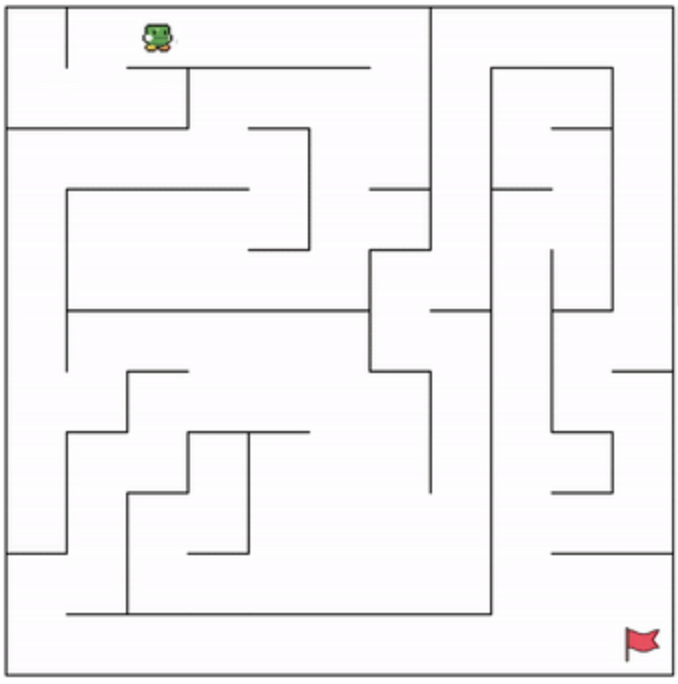
\includegraphics[width=0.27\textwidth]{mazepic.png}
  \vspace{-0.85cm}
\end{wrapfigure}
In CS 660/760, my classical artificial intelligence course (UAB had six courses focused on machine learning), we used the Russell-Norvig book and other standard material, but I also invested significantly in developing new material myself and did quite a bit of live coding in class to illustrate key algorithms. For example, I would spend an entire one-and-a-half lectures developing a Sudoku solver when first introducing the idea of CSP and SAT problems, using a Socratic and interactive pedagogical approach to coax the solution gradually out of students. \textbf{I knew the typical mistakes students would make and could allow us to take wrong turns so we would learn together from the experience of discovering these issues and solving them live, in class together}. I focused on planning, heuristics, optimization, constraint solving, logic, SAT, DPLL, CDCL, and SMT, and in 2024 I replaced a unit (that I originally made in 2019) on minimax game playing where students built Reversi players with a unit where \textbf{students built adversarial agents playing a simulated capture-the-flag game}, which I found generated a lot of productive engagement among students. I built the game as a C++ server (available on GitHub\footnote{\url{https://github.com/harp-lab/maze-game}}) that would connect to one or two players (as subprocesses), accepting real-time moves and rendering out a video (a still image from the introductory single-player version of the game is shown above). On the last day of class we watched a tournament of all the class robots battling it out and discussed what worked well and what didn't.

Finally, CS 401/501 was a programming languages (PL) course I developed from scratch, based on my experience teaching CMSC 330 at UMD combined with some elements I liked from other courses I've taken, or read curriculum for online, and some of my own ideas. I wanted to combine a survey-of-paradigms approach (as used at UMD) with a greater emphasis on functional programming and add a touch of formal semantics and material on writing practical interpreters---\textbf{a focus that stems from my pedagogical philosophy that building a system from scratch} (in this case a language, via several different kinds of interpreters) \textbf{is a powerful route to learning}, an approach that works particularly well in computer science where engineering an end-to-end artifact can be an accessible class project. As a fan of the Friedman-Wand textbook who had several opportunities to chat with Dan Friedman (and two of his PhD students) about his Indiana U. PL course, I imbued a lot of his perspective on writing a series of bite-sized interpreters, each with a small delta, to illustrate a progression of features, into my course.

\colorbox{lightgray}{\textbf{At WSU:}} CptS 452 is a completely new \emph{``Compilers''} course I've developed here at WSU. This is an important subject for me as it's the one that originally sparked a deep interest in computer science and programming languages. I plan to grow this course into a unique experience for WSU students that will empower them to become better programmers through both a hands-on peek under the hood of modern PL implementations and guided classroom experience building a large integrated project. My approach is informed by several closely related perspectives: Matt Might's compilers course at the University of Utah (for which I helped develop tests and reference materials), the Siek-Newton textbook which does a phenominal job leveraging the nano-pass compiler architecture for teaching compilers one small functional pass at a time, and innumerable discussions I had with Andy Keep (from our shared time at Utah) whose dissertation rebuilds the (state-of-art) Chez Scheme compiler using a macro-based approach for instantiating nano-pass-style functional compilers. In my first iteration teaching this new course, I taught Scheme and had \textbf{every student compile Scheme to C, in Scheme, as a series of small passes} that desugar the language to a core intermediate language, compile the stack to functions using continuation passing, and then compile functions to objects using bottom-up closure conversion. I have plans to significantly improve this project that I explore below, but wanted to keep it streamlined for the initial offering. I taught a number of elective topics separately from the project, some of which I would ideally include within the class project: garbage collection, register allocation, dataflow analysis, and flow-directed optimization.

CptS 580 is a completely new and unique graduate-level \emph{``Advanced Programming Languages''} course \textbf{that focuses on reasoning formally about programs and language features}. As CptS 355 teaches a survey of language paradigms, I want to focus our graduate-level PL course on language semantics, interpreters, and formal methods. Perhaps the most helpful course I took in my own PL education was Matthew Flatt's graduate \emph{``Semantics''} class, an absolutely fantastic tour of formal semantics and modeling that taught me so many of the tools I would go on to apply in my research. It also gave me the conceptual framework to understand more precisely how languages work and how different features would interact. My vision for the first half of class is to orient students to the major branches of formal semantics, focus in on operational semantics by teaching the lambda calculus and systematically building up structural and natural semantics in small steps: we may eliminate capture-avoiding substitution with the explicit structure of binding environments, we may eliminate reduction contexts and natural deduction with explicit stack passing, as in Kriven's machine, etc. Following my focus on practical programming projects, I pair these theoretical developments with practical coding projects where each style of interpreter is implemented, either in class or as an exercise. In the second half of the class, I segue from natural semantics to natural deduction and type systems, introducing the connection to intuitionistic logic and modern theorem provers. Finally, we explore let polymorphism and two influential approaches to program analysis (summarization and abstract interpretation), using a classic paper from the literature to introduce each.


\paragraph{Teaching Vision for WSU}

I plan on developing \textbf{a world-class PL curriculum at WSU} that dovetails with our existing strengths in software engineering, security, and artificial intelligence. To accomplish this, I will further develop and crystalize my vision for CptS 452 as an exciting, practical, and engineering-oriented course students will love that focuses explicitly on building as large and realistic an end-to-end compiler as 400-level students can reasonably manage---gracefully scaling up or down with elective components to suite a student's ambition and interests. One that brings a deep conceptual toolbox into our students' awareness and leaves them empowered as programmers, whether or not they end up building any compilers or language-related tooling in their careers. I have too many ideas to condense here properly, but will call out a few I plan to explore: (a) providing a black-box implementation of all compiler passes to improve student-lead capacities for test-driven development, (b) extending the front end with Python-like features and syntax, (c) extending the back end with lower-level optimizations and target LLVM IR, WASM, or x86. Although I wouldn't push for any specific changes to other courses, I have had some conversations with Subu Kandaswamy about aligning CptS 580 and 355 (undergrad PL) and I think there will be key opportunities as well with CptS 317 (automata). For example, if CptS 317 does not teach parsing in practice, then extension (b) would be a nice way to include this material in CptS 452; if CptS 355 taught Scheme, and certain FP concepts, these would be easier to assume in CptS 452.


\paragraph{Mentoring Philosophy}

My mentoring philosophy centers around two main ideas: that students need to build their skillset in managable concrete layers, and that \textbf{the best way to learn a complex topic is to understand and replicate the state of the art}. I typically begin working with students by bringing them up to speed on foundational topics in my area, finding out what recent ideas are most exciting to them, and guiding my student to rebuild this state of art themselves. As a student gains practical confidence in a core topic, I will assign papers further afield to read and discuss with me, add a secondary project, and have the student collaborate or mentor another more junior student. 

I feel strongly that a PhD student learns from a wide variety of influences in their lab and department, not only their advisor---my own best influences and resources in grad school were frequently the postdocs and other PhD students in the lab. I endeavor to ensure my students are supporting one another and constantly in a position to collaborate and learn from one another. My PhD students always have both a primary research project, along with supporting roles on other projects for which they are not primarily responsible. I also assign PhD students as mentors to my BS and MS students so that in addition to their meetings with me, the junior student also meets privately with a PhD student at least once a week. This provides the junior student another sounding board who they might feel more open to seeking certain kinds of help from, and as teaching can often be the most effective method for learning, provides the more senior student with a valuable experience communicating ideas they've recently learned with clarity.%enough clarity to support someone still new to those ideas.

\paragraph{Mentoring Experience}

I have experience \textbf{advising five PhD students, graduating one} (Ke Fan, now Assistant Professor at Temple University). My next most senior PhD student (Ahmedur Rahman Shovon, co-advised by Sidharth Kumar at UIC) plans to defend summer term 2025. Another PhD student (Sowmith Kunapaneni) has joined me at WSU after starting at UAB, has published at VLDB this year, has a paper in submission at SC (Supercomputing), and has a first-author paper in preparation to be submitted to a VLDB or SIGMOD deadline this summer. Another student (Akash Rao) started this last year and already has a first-author paper currently in submission to SC (co-authored with Sowmith). Last, a new PhD student (Henry Olson) is joining my lab this upcoming year and we have been meeting regularly on Zoom since February to get him up to speed on a several important background topics.

I have also been a mentor and committee member for four other PhD students, two of whom I have worked with especially closely and published with multiple times each, including at top venues VLDB, ASPLOS, and AAAI. I have further graduated two MS students, one who published an EduHiPC paper on his Thesis topic, and am currently working with two MS Thesis students here at WSU, one who is developing a thesis topic related to compiling functional languages after taking my \emph{``Compilers''} course. %this last fall. Below I highlight a few notable mentoring experiences.

\textbf{Ke Fan} and Kyle Headley were the first two PhD students to join my lab in 2019. (Kyle quickly left his PhD at the start of the pandemic to be with family and take an industry position.) Ke Fan worked closely with both Sidharth and I as co-advisors on our joint work to scale iterated joins for Datalog using MPI, joining us for virtually every collaborative meeting we had in 2020 over Zoom. I would individually mentor Ke on Datalog and the structure of our algorithm, while Sidharth did the same for a series of classical MPI algorithms we wanted to draw inspiration from. She quickly honed in on our all-to-all communication phase, a unique feature of our approach that had unusual characteristics (i.e., low-volume variadic all-to-all with strict latency requirements). Within two years \textbf{she wrote an HPDC paper developing a novel variant of the Bruck algorithm} to suite these requirements, showing its scalability and developing a performance model. She joined Sidharth when he moved to from UAB to UIC in 2023 and went on to publish with us at ICS. \textbf{She has since graduated and joined Temple University} (as Asst. Prof).

\textbf{Ahmedur Rahman Shovon} joined my lab in late 2021 after the pandemic, co-advised by Sidharth and I, focusing on GPU implementations of relational joins. I worked especially closely with Shovon in his first year to help him master GPU programming (something I've been involved with since my work on GPU-based iterated SpMM with Jim King in 2016). At first this was challenging given Shovon's background and required much pair programming and concrete-task development on my part. I decided we would start with a workshop paper comparing a basic implementation to cuDF, which was published at IA3, with a follow-up at USENIX ATC. I have found lower-pressure workshop submissions are the best way to start a student on publishing. Around this time, Shovon opted to move with Sidharth to UIC in 2023. After this success comparing a customized hash-join algorithm with cuDF, I integrated Shovon into a collaborative project with my colleague at Syracuse (Kris Micinski) and his PhD student (Yihao Sun). With Yihao, Kris and I had been developing a new approach to performing joins on the GPU using a novel three-layer data structure to reduce thread divergence, coalesce memory accesses, and optimize various aspects of the algorithm. \textbf{Shovon co-authored a paper at ASPLOS with Yihao and went on to publish a first-author paper at ICS} on scaling multi-node, multi-GPU joins. I am currently working with Shovon and my student Sowmith to study the power requirements of this and related algorithms, aiming to submit to ASPLOS. We are currently scheduling Shovon's PhD defense at UIC for this summer. 

\textbf{Sowmith Kunapaneni} started working with me as an MS student at UAB who took my CS 501, \emph{``Programming Languages''} class and has some novel ideas related to lazy datastructures after a lecture on Okasaki queues. I integrated him into a group of other BS and MS students I was working with to devleop a compiler. (UAB did not offer an official ``Compilers'' course, so I would regularly work with a group of interested students to teach this topic informally or as an independent study.) Sowmith became interested in compilers, abstract interpretation, Datalog, GPU programming, and other topics I could teach him and converted to a PhD student in my lab officially after a year in the MS program. At this point I integrated him into my Slog project, a theory and implementation of Datalog with first-class facts to explore monotone data-parallel functional programming. He helped us improve some of our experiments and \textbf{co-authored an improved draft of this work that was accepted at VLDB 2025}. He joined me in moving to WSU where he assisted a new PhD student \textbf{Akash Rao}, recommended by my collaborator Ananth Kalyanaraman, in developing an idea for parallel-prefix-based iterated joins in MPI that avoids communication entirely. Akash and Sowmith submitted a paper at SC (Supercomputing) this year. At the same time, Sowmith has been developing a vectorized implementation of Yihao and Shovon's GPU-based joins and investigating approaches to worst-case-optimal joins; he has work in preparation to be submitted at either VLDB or SIGMOD this summer.


\paragraph{Student Evaluations}

I always pay close attention to feedback from students, whether in person or anonymous, officially solicited or unsolicited, and make adjustments in response. Some unsolicited course evaluations from UMD students and UAB students may be found on \href{https://planetterp.com/professor/gilray}{PlanetTerp.com} and \href{https://www.ratemyprofessors.com/professor/2399194}{RateMyProfessor.com} respectively. I'm proud to have received \emph{repeated} comments saying mine was \emph{``the best course I've taken''} and \emph{``[Tom is] the best professor I have had''}.  I am attaching my last term's course evaluations.

%% \begin{itemize} \tiny \setlength\itemsep{-0.7em} \itshape
%% \item I greatly appreciate the time and effort Dr. Gilray puts into his lectures and assignments. With his guidance, and well asked questions by myself and other students, it is unlikely that I ever left any lecture with a misunderstanding or missing piece of information relevant to the material. Additionally, he does an excellent job of providing extra related material for further study, which is very valuable.
%% \item I think Professor Gilray is the best professor I have ever had. His courses are very challenging, but he always provides excellent resources and is sure to set us up for success. His lectures are organized, thought-out, interesting, and a joy to attend. It was a shame that we had to continue the semester online after spring break, but he still provided lecture videos and other materials online for us to learn from. His recorded lectures were just as engaging as in-person lectures and we could tell a lot of work was put into them, which is no surprise. All coding assignments were interesting, and some very difficult, but the autograder was a priceless resource. He also always made sure we knew we could contact him for any help and offers excellent guidance. I am so grateful I got to take 2 courses (CS350 and CS401) under him. Thank you, again, Professor Gilray for a great semester!
%% \item I found Professor Gilray’s lectures to be interesting and well put together. It’s rare to find a Professor as passionate as he is about the topic they are teaching. I think that’s what made me never want to miss a class. This class was extremely challenging, probably the most difficult class I have ever taken, but I think I learned much more than I have in any other class. I thoroughly enjoyed the programming projects, especially building the parser, and the assignments helped solidify the material for me. The only negative thing I have to say is that I think the tests were a bit too long. I wasn’t able to finish either of the two midterms, and I feel like I am usually a good test taker. Perhaps I didn’t study enough, as I know some students did exceptionally well, but I’ll be sure to study much more for the final! Thank you Professor Gilray and I’m looking forward to 401 in the spring.
%% \item Excellent lecture! Well structured, I have no difficulty in understanding the course. Also, Autograder is excellent! You can see your result right away, which is very efficient. I hope this system can be promoted to other classes for code submission as well.
%% \item This is the best course I've taken at UAB.
%% \item The midterm review was greatly appreciated along with the exam closely following the material covered in the review session.
%% \item The difficulty of the class was well compensated for by the amount of bonus opportunities provided. Great job!
%% \end{itemize}
 


\end{document}
